
\lyxframeend{}\section{ROS}


\lyxframeend{}\subsection{ROS Introduction}


\lyxframeend{}\lyxframe{ROS Introduction}

ROS
\begin{itemize}
\item Meta Operating System for robotics
\item Obtain, build, write and run code across multiple computers and robots
\item Open Source
\item BSD Licensed (very liberal%
\footnote{\href{http://en.wikipedia.org/wiki/BSD_licenses}{http://en.wikipedia.org/wiki/BSD\_{}licenses}%
})
\item Willow Garage
\item Community
\end{itemize}

\lyxframeend{}


\lyxframeend{}\lyxframe{Introduction (cont.)}


\framesubtitle{Robots Using ROS > 50}

\noindent \begin{center}
\begin{figure}[H]
\noindent \centering{}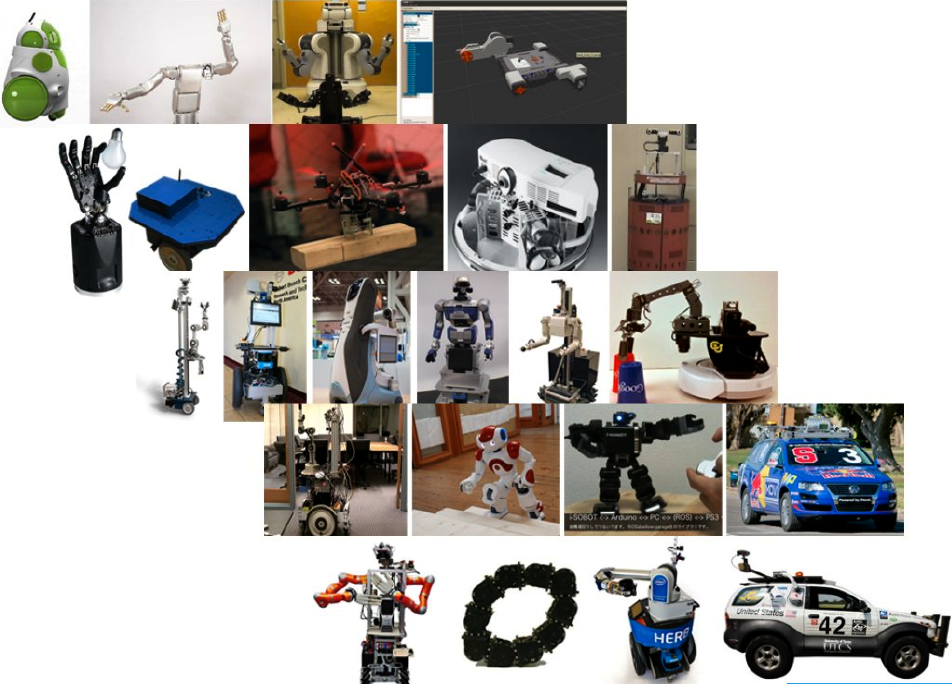
\includegraphics[bb=0bp -160bp 952bp 480bp,height=0.8\paperheight]{images/ROSManyRobots}
\end{figure}

\par\end{center}


\lyxframeend{}


\lyxframeend{}\lyxframe{ROS Basics}
\begin{itemize}
\item Supported Platforms

\begin{itemize}
\item Linux, Mac OS, partial support for Windows
\end{itemize}
\end{itemize}

\pause{}
\begin{itemize}
\item Languages

\begin{itemize}
\item C/C++, Python, Octave, Lisp, Java
\end{itemize}
\end{itemize}

\lyxframeend{}


\lyxframeend{}\lyxframe{What does ROS cover?}

ROS
\begin{itemize}
\item Simulation
\item Task execution
\item Mobile manipulation
\item Navigation
\item Visualization
\item Client libraries
\item Message passing
\end{itemize}

\lyxframeend{}


\lyxframeend{}\subsection{ROS Concepts}


\lyxframeend{}\lyxframe{ROS Nodes}
\begin{itemize}
\item Master (rosmaster)

\begin{itemize}
\item provides naming and registration services
\item tracks topics and services
\item enables localization of nodes (nodes talk peer-to-peer)
\item XML-RPC-based API
\end{itemize}
\item Generally: they are uniquely named
\end{itemize}

\lyxframeend{}


\lyxframeend{}\lyxframe{[allowframebreaks]ROS Communication}
\begin{itemize}
\item Publisher sends message to subscribers

\begin{itemize}
\item Usually TCP/IP transport
\item XML-RPC is only used to negotiate transport (no messages via XML-RPC)
\end{itemize}
\end{itemize}
\noindent \begin{center}
\begin{figure}[H]
\noindent \centering{}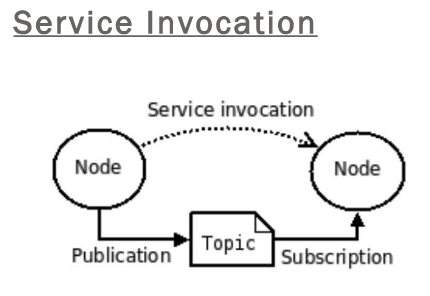
\includegraphics[width=0.45\textwidth]{images/ServiceInvocation}
\end{figure}

\par\end{center}


\lyxframeend{}


\lyxframeend{}\lyxframe{ROS Communication (cont.)}

\noindent \begin{center}
\begin{figure}[H]
\noindent \centering{}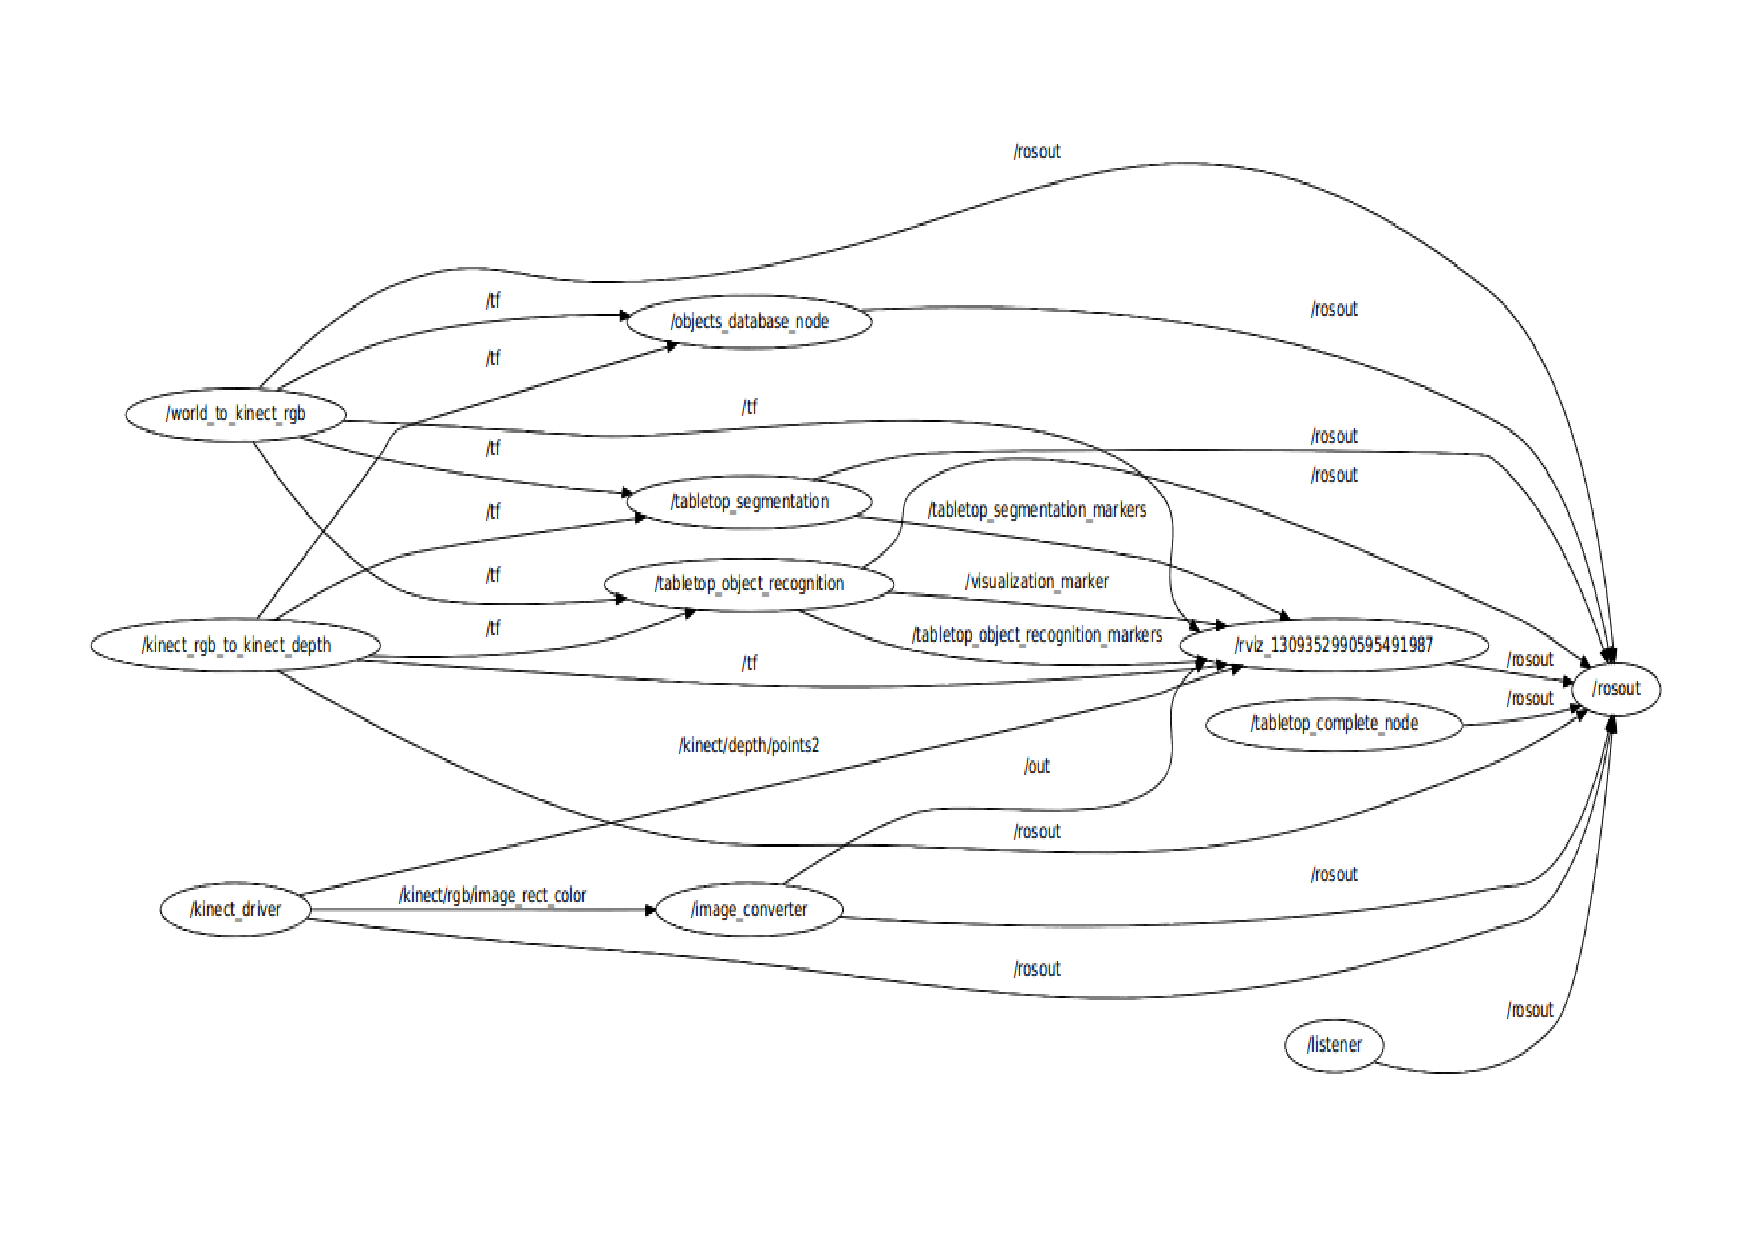
\includegraphics[bb=40bp 0bp 800bp 530bp,clip,width=1\textwidth]{images/ros_rxgraph}
\end{figure}

\par\end{center}


\lyxframeend{}


\lyxframeend{}\subsection{ROS Repositories}


\lyxframeend{}\lyxframe{ROS Repositories}

Repositories world-wide
\begin{itemize}
\item Collection of packages and stacks, hosted online
\item many repositories (>50): Stanford, CMU, TUM ..
\end{itemize}
\noindent \begin{center}
\begin{figure}[H]
\noindent \centering{}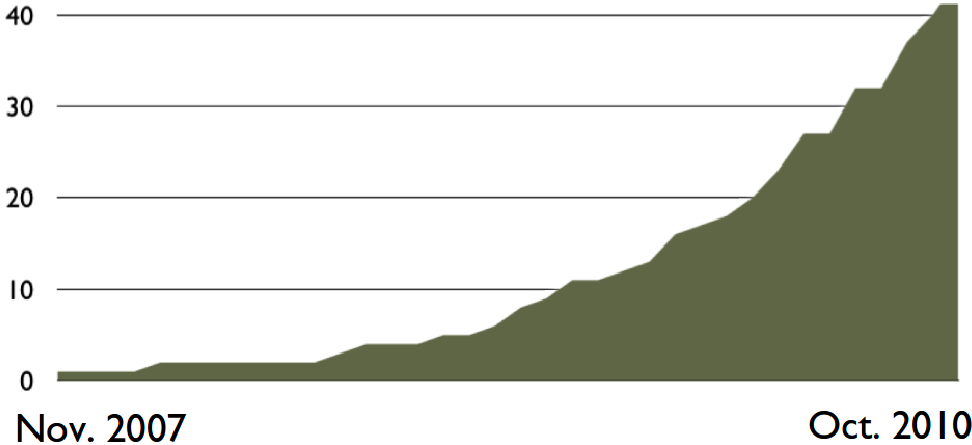
\includegraphics[width=0.9\textwidth]{images/ROSReopGrowth}
\end{figure}

\par\end{center}


\lyxframeend{}


\lyxframeend{}\lyxframe{ROS Repositories (cont.)}

\noindent \begin{center}
\begin{figure}[H]
\noindent \centering{}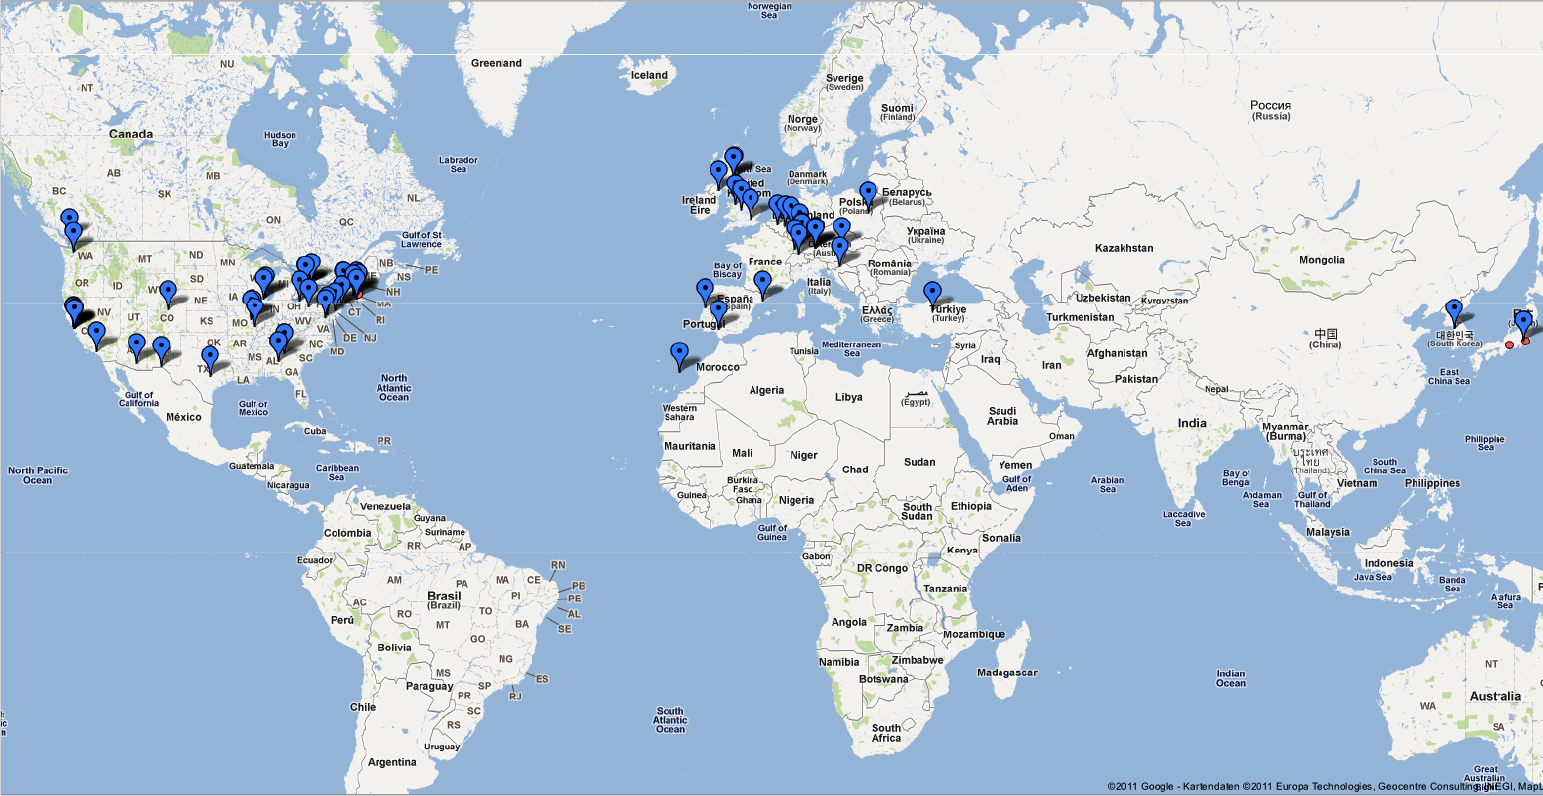
\includegraphics[bb=80bp 0bp 1350bp 550bp,width=1\paperwidth]{images/ROS_Repositories}
\end{figure}

\par\end{center}


\lyxframeend{}


\lyxframeend{}\lyxframe{ROS Stacks}
\begin{itemize}
\item Collect similar packages that work together to achieve e.g.:

\begin{itemize}
\item 2D Navigation
\item Manipulation
\item SLAM
\end{itemize}
\end{itemize}
\noindent \begin{center}
\begin{figure}[H]
\noindent \centering{}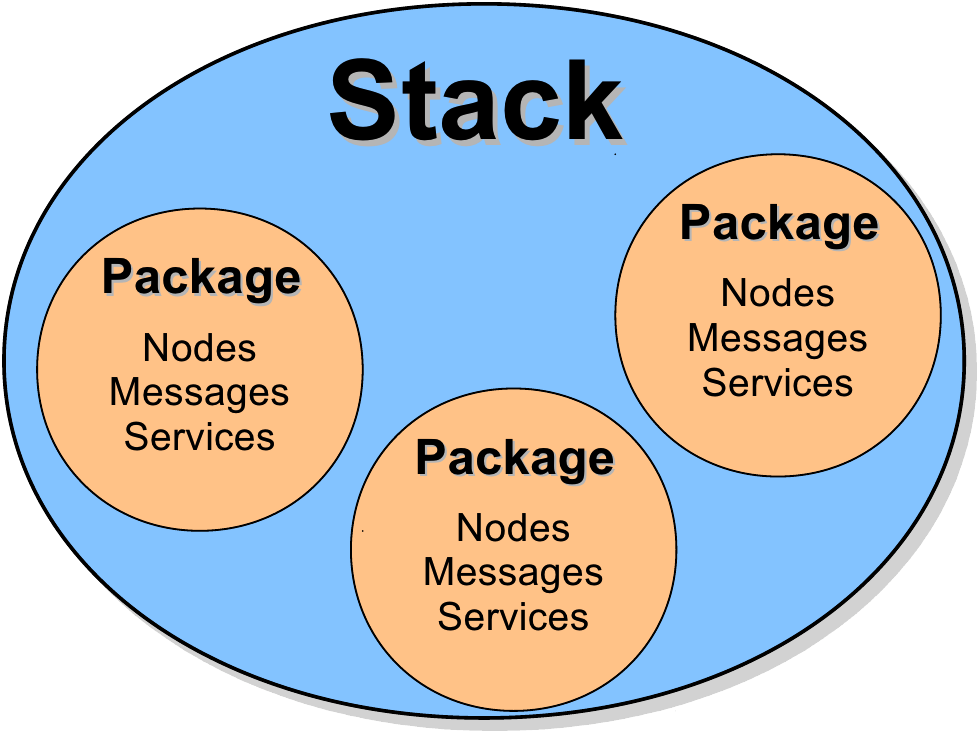
\includegraphics[width=0.45\textwidth]{images/ROSStack}
\end{figure}

\par\end{center}


\lyxframeend{}


\lyxframeend{}\lyxframe{ROS Stacks Overview%
\footnote{\href{http://www.ros.org/browse}{http://www.ros.org/browse}%
}}


\framesubtitle{Currently > 400 Stacks available}

\begin{minipage}[t]{0.45\textwidth}%
\begin{itemize}
\item (2D/3D) Navigation 
\item PR2 arm navigation
\item PR2 opening doors 
\item Exploration
\item GUI for PR2 robot
\item PR2 object manipulation 
\item PR2 simulator\end{itemize}
%
\end{minipage}%
\begin{minipage}[t]{0.5\paperwidth}%
\begin{figure}[H]
\noindent \centering{}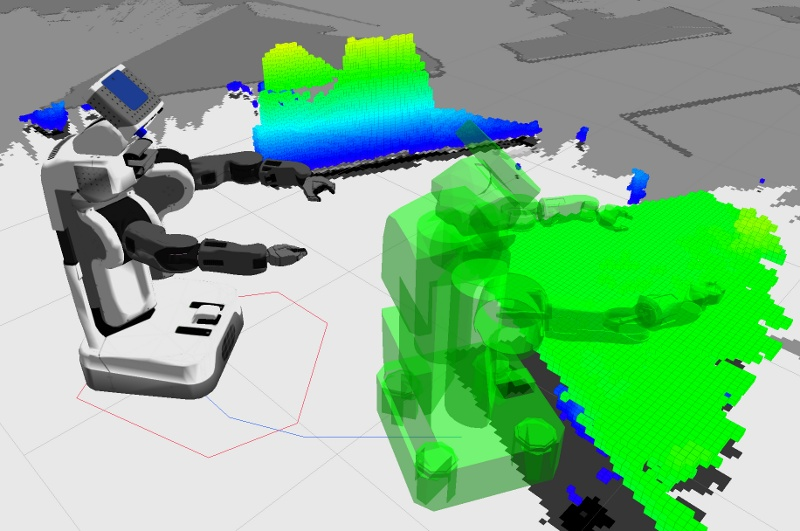
\includegraphics[height=0.4\textheight]{images/PR2_3DNavigation}\\
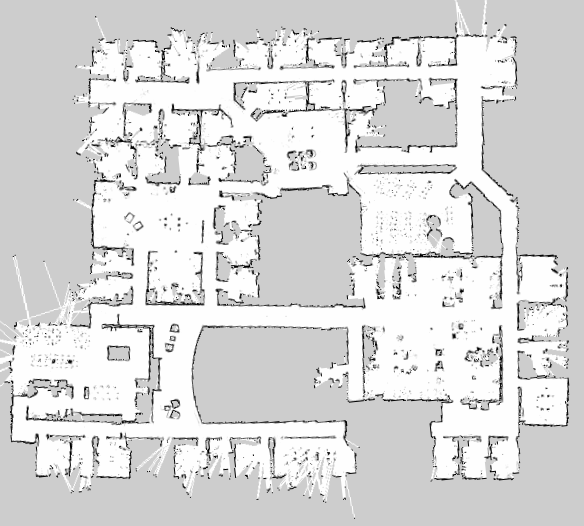
\includegraphics[height=0.2\textheight]{images/2DMapping}\includegraphics[height=0.2\textheight]{\string"images/PR2 Opening doors\string".png}
\end{figure}
%
\end{minipage}


\lyxframeend{}


\lyxframeend{}\lyxframe{ROS based Navigation}

Includes
\begin{itemize}
\item Path planning, Obstacle avoidance, Automatic map making
\end{itemize}
\noindent \begin{center}
\begin{figure}[H]
\noindent \centering{}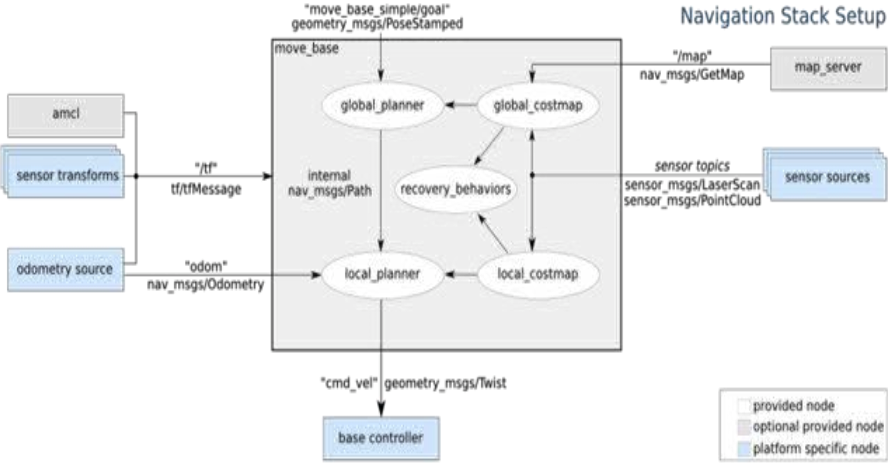
\includegraphics[width=0.9\textwidth]{images/ROSNavigation}
\end{figure}

\par\end{center}


\lyxframeend{}


\lyxframeend{}\lyxframe{[allowframebreaks]Example Application}

\noindent \begin{center}
\begin{figure}[H]
\noindent \centering{}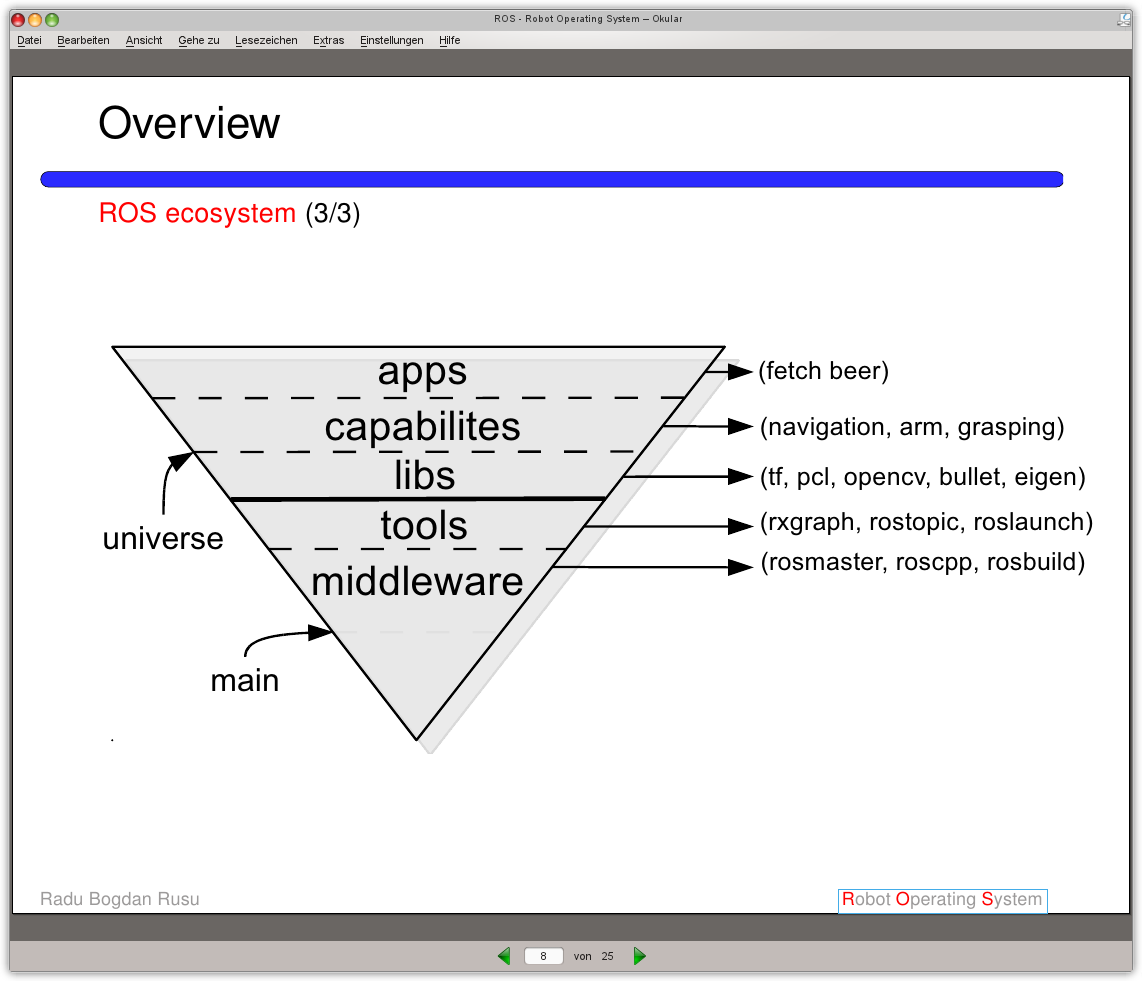
\includegraphics[width=1\textwidth]{images/ROSEcosystem}
\end{figure}

\par\end{center}

\noindent \begin{center}
\begin{figure}[H]
\noindent \centering{}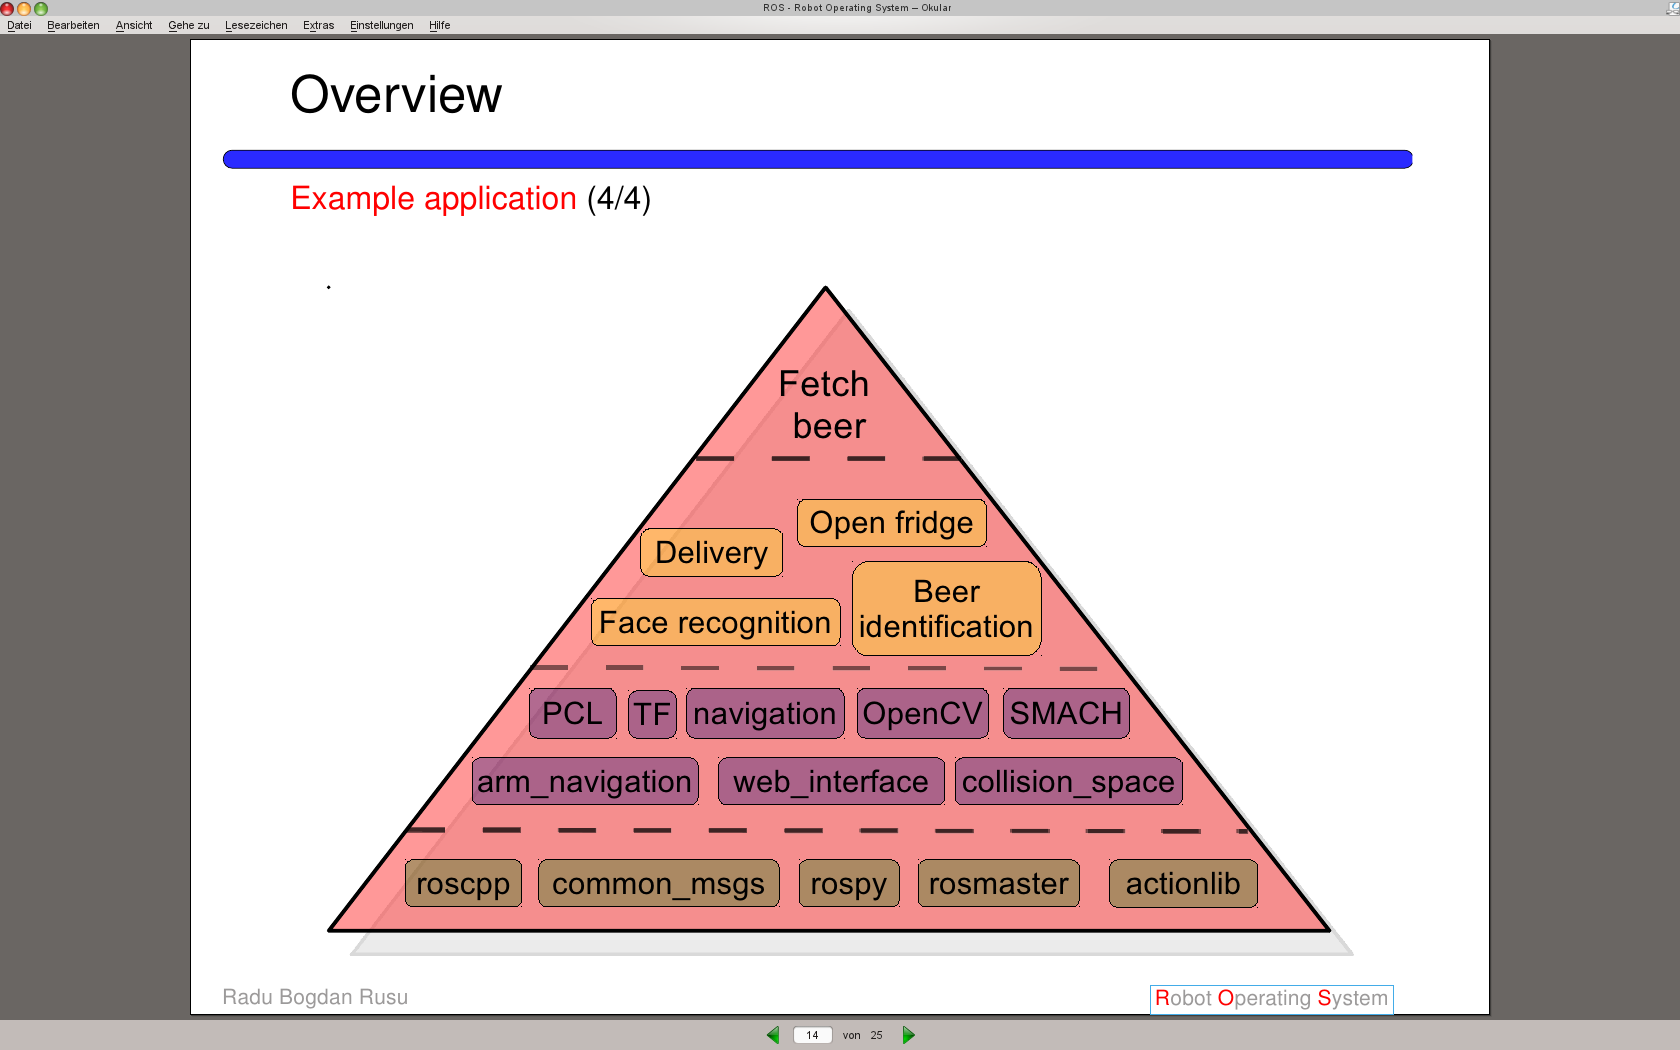
\includegraphics[width=0.9\textwidth]{images/ROSFetchBeer}
\end{figure}

\par\end{center}


\lyxframeend{}


\lyxframeend{}\lyxframe{ROS Strengths for RACE}
\begin{itemize}
\item Visualization
\item Object recognition
\item Navigation
\item Manipulation/Grasping
\item Plugging in Sensors

\begin{itemize}
\item already integrated
\item RACE specific
\end{itemize}
\end{itemize}

\lyxframeend{}
